\section{Semana 7 - Fuselagem Design, Design Point Iteration}

\subsection{Introdução}
A semana 7 focou-se principalmente no design da fuselagem. Procurando-se ter valores concretos para as dimensões exteriores desta mesma, nomeadamente, o comprimento total e a largura. Além disto, também o interior foi concebido, focando-se na colocação dos assentos, portas, material médico, \textbf{inserir mais coisas}. Este último foi largamente baseado no AW 139.\par
O segundo objetivo da semana foi realizar iterações do design point a fim de encontrar valores que resultassem num melhor design. Para tal foi desenvolvido um programa em python que lê o json do design e aplica um algoritmo genético simples para chegarmos a um design melhor. De forma a poder automatizar a criação de novos designs, bem como a sua avaliação com o programa em python e gerar o desgin point em matlab, necessário para o algoritmo genético, foi escrito um script em poweshell. Além disto, o programa em matlab original foi modificado a fim de ser possível retirar as coordenadas do design point a fim de serem utilizadas pelo programa em python. 
\subsection{Fuselage Design - Exterior}
\subsection{Fuselage Design - Interior}
\subsection{Iteration}
A iteração foi implementada em powershell e teve a seguinte forma.:\vspace{5pt}
\FloatBarrier
\fbox{
    \begin{minipage}{\textwidth}
        \begin{itemize}
            \item Correr programa de inicialização/geração inicial de novos ficheiros json com ficheiro original como imput
            \item Fazer loop n vezes
            \begin{itemize}
                \item Correr matlab para todos os ficheiros gerados
                \item Correr programa python com algoritmo genético
            \end{itemize}
        \end{itemize}
    \end{minipage}
}
\FloatBarrier
\vspace{5pt}
O programa de inicialização tem a seguinte estrutura:
\vspace{5pt}
\FloatBarrier
\fbox{
    \begin{minipage}{\textwidth}
        \begin{itemize}
            \item Abre o ficheiro json que recebe como imput
            \item Corre n vezes
            \begin{itemize}
                \item Varia as seguintes variaveis por um valor entre $\pm0.1\% e \pm1\%$
            \begin{itemize}
                \item fuselagem - diametro
                \item asa - aspect ratio, corda média
                \item rotor - raio, rotor\_solidity
            \end{itemize}
            \item Cria ficheiro json n
            \end{itemize}
            
        \end{itemize}
    \end{minipage}
}
\FloatBarrier
\vspace{5pt}
O programa matlab corre os 10 ficheiros json criados, e gera um ficheiro de texto com as coordenadas dos design points (W/P,W/A) e (W/P,W/S) de cada json gerado.
O segundo programa escrito em python, com o algoritmo genético, tem a seguinte estrutura:
\vspace{5pt}
\FloatBarrier
\fbox{
    \begin{minipage}{\textwidth}
        \begin{itemize}
            \item Abre o ficheiro com as coordenadas dos designs points dos 10 designs gerados
            \item Calcula a figura de mérito para cada design
            \item Preserva o ficheiro com melhor figura de mérito; apaga o resto
            \item chama o programa de inicialização com ficheiro com melhor figura de mérito como input
        \end{itemize}
    \end{minipage}
}
\FloatBarrier
\vspace{5pt}
O cálculo da figura de mérito é feito através do seguinte algoritmo
\vspace{5pt}
\FloatBarrier
\fbox{
    \begin{minipage}{\textwidth}
    \begin{itemize}
        \item Se a coordenada x de (W/P, W/S) <=1300 e a coordenada y de (W/P, W/A) <=6000
        \begin{itemize}
            \item Mérito = 1/(coordenada x de (W/P, W/S))+10*(coordenada y de (W/P, W/A))
        \end{itemize}
        \item else
        \begin{itemize}
            \item Mérito = 0
        \end{itemize}
    \end{itemize}
    \end{minipage}
}
Este algoritmo tenta puxar o ponto (W/P, W/S) para a esquerda e o ponto (W/P, W/A) para cima, encontrando um equíbrio entre os dois.\par
O código de inicialização tem a seguinte forma. Aoesar de ser pouco prático de editar e poder ser feito uma implementação com loop, a falta de conhecimento sobre a linguagem python levou a que esta solução fosse criada, dado os ganhos de tempo em não aprender formas mais compactas e editáveis numa nova linguagem de programação.\par
\vspace{5pt}
\hrule
\vspace{5pt}
\FloatBarrier

    \begin{minipage}{\textwidth}
        \begin{minted}{python}
        import json
        import random
        import sys
        print(sys.argv[1])
        print()
        a_file = open(str(sys.argv[1]), "r")
        json_object = json.load(a_file)
        random.seed(a=None, version=2)
        a_file.close()
        #print(data)
        for i in range(10):
            json_object['vehicle']['components'][4]['diameter'] += random.randrange(10)/1000*json_object['vehicle']['components'][4]['diameter']*(random.randint(0,1)*2-1)
            json_object['vehicle']['components'][5]['aspect_ratio'] += random.randrange(10)/1000*json_object['vehicle']['components'][5]['aspect_ratio']*(random.randint(0,1)*2-1)
            json_object['vehicle']['components'][5]['mean_chord'] = json_object['vehicle']['components'][5]['aspect_ratio']/7
            json_object['vehicle']['components'][7]['aspect_ratio'] += random.randrange(10)/1000*json_object['vehicle']['components'][7]['aspect_ratio']*(random.randint(0,1)*2-1)
            json_object['vehicle']['components'][7]['mean_chord'] += random.randrange(10)/1000*json_object['vehicle']['components'][7]['mean_chord']*(random.randint(0,1)*2-1)
            json_object['vehicle']['components'][13]['radius'] += random.randrange(10)/1000*json_object['vehicle']['components'][13]['radius']*(random.randint(0,1)*2-1)
            json_object['vehicle']['components'][13]['rotor_solidity'] += random.randrange(10)/1000*json_object['vehicle']['components'][13]['rotor_solidity']*(random.randint(0,1)*2-1)
            #json_object['vehicle']['components'][13]['number'] += round((random.randint(0,1)-0.65))
            #json_object['vehicle']['components'][17]['number'] = json_object['vehicle']['components'][13]['number']
            with open('JSONS/data'+str(i)+'.json', 'w', encoding='utf-8') as f:
                json.dump(json_object, f, ensure_ascii=False, indent=4)
        \end{minted}
    \end{minipage}

\hrule
\vspace{20pt}
O código que calcula a figura de mérito é o seguinte:\par
\vspace{2pt}
\hrule
\vspace{5pt}
\FloatBarrier
\begin{minted}{python}
import csv
import os

meritList = []

class merit:
    val = 0
    def calc(me,a,b):
        if a <= 1300 and b <= 6000:
            me.val=1/(a)+(10*b);
        else:
            me.val=0
        
MyMerit=merit()

with open('design_points.txt', newline='') as csvfile:
    points = list(csv.reader(csvfile, delimiter=',', quotechar='|'))
    print(points[1][1])
    print()
    i=0;
    for row in points:
       MyMerit.calc(float(points[i][0]),float(points[i][3]))
       print(MyMerit.val)
       i=i+1
       meritList.append(MyMerit.val)

for k in [x for x in range(i) if x != meritList.index(max(meritList))]:
    os.remove('JSONS/data'+str(k)+'.json')

os.system("py eddit_vars.py"+' JSONS/data'+str(meritList.index(max(meritList)))+'.json')

\end{minted}

\hrule
\vspace{20pt}
O script de powershell é o seguinte:
\vspace{2pt}
\hrule
\vspace{5pt}
\FloatBarrier
\begin{minted}{powershell}
py eddit_vars.py "JSONS/prototipo3_funciona.json"
foreach($i in 1..10){
matlab -nosplash -nodesktop -r "run('ARChanges_runtrhough_underscores.m')";
Start-Sleep -Seconds 35
py secondpart_edit_vars.py
}
\end{minted}
\hrule
\vspace{20pt}
Esta implementação permitiu rapidamente passar dum design para um outro considerado melhor. É apresentado o antigo e novo design de forma a mostrar os avanços desta semana em relação ao design point.\par
\FloatBarrier
\begin{figure}[h]
        \centering
    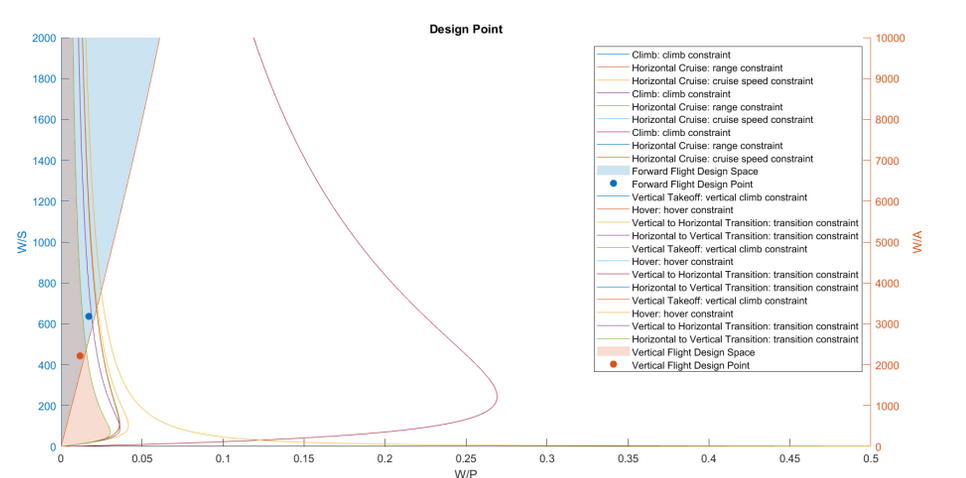
\includegraphics[width=\textwidth]{Imagens/json_1_semana7.PNG}
    \caption{Design Antigo}
    \label{json_1_semana7}
\end{figure}
\FloatBarrier
\begin{figure}[h]
     \centering
    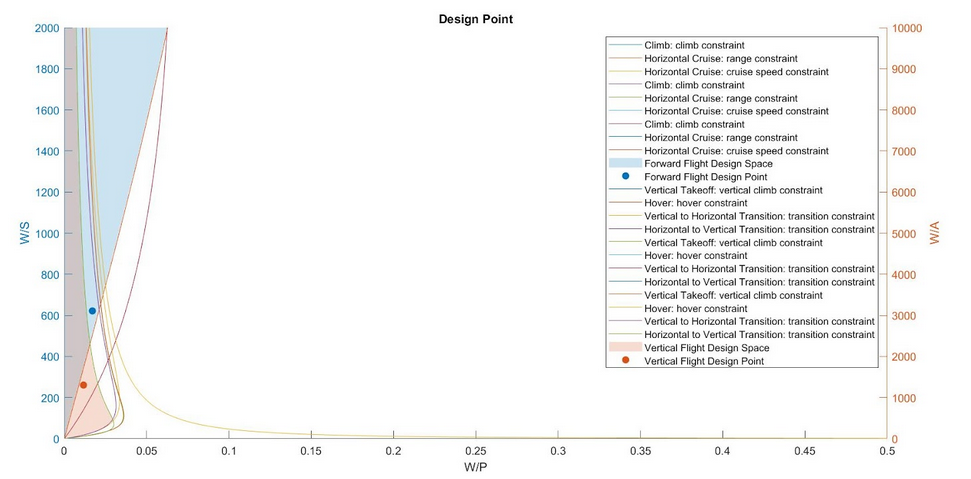
\includegraphics[width=\textwidth]{Imagens/json_2_semana7.PNG}
    \caption{Novo Design - Semana 7}
    \label{json_1_semana7}
\end{figure}
\FloatBarrier